\documentclass[answers,addpoints]{exam}
\usepackage{amsmath,amssymb,enumerate,float,tikz,etoolbox,ifthen,xcolor,fullpage,ulem,graphicx, comment,hyperref,multicol,enumerate,makecell,pgfplots}
\pgfplotsset{compat=1.18} % overleaf suggestion
\usetikzlibrary{decorations.pathreplacing}

\definecolor{MyGreen}{rgb}{0.1, 0.4, 0.1}
\definecolor{MyBlue}{rgb}{0.1, 0.1, 0.9}

\AtBeginEnvironment{solution}{\color{MyGreen}}

\newboolean{NoSolutions}

\usepackage{tagging}

\noprintanswers
\printanswers

\newcommand\pts[1][2]{\textcolor{MyBlue}{\text{\bf [#1 pts]}}}
\newcommand\pt{\textcolor{MyBlue}{\text{\bf [1 pt]}}}

\setlength\parindent{0in}
\pagestyle{empty}
\begin{document}

\section*{MATH 100 GROUP PROJECT 1: Limits and Asymptotics}

Alexandre \textbf{Boutoille} (22291660)

Brennan \textbf{Coetzer} (64702178)

Dino \textbf{Lee} (29709300)

Andaya \textbf{Vincent} (33234436)

\normalsize

\

{{In this project, you will explore how functions behave when $x$ is very small (generally meaning $x \to 0$ but we will sometimes focus on $x \to 0^+$ to include functions like $\log(x)$ or $\sqrt{x}$ in our explorations) and when $x$ is very large ($x \to \infty$). You will compare functions from different families such as polynomials, roots, logarithms, exponentials, and combinations of these and determine which terms or factors dominate in each regime.}

  \

  {This type of thinking is central to understanding limits and asymptotics in calculus. It allows you to make clear qualitative statements about growth, decay, and oscillation, and to compare functions without relying on detailed algebraic manipulations. The focus will be on describing behaviours and relative sizes, supported by reasoning and graphs.}
}

\

Your group submission must be typed, and marks will be awarded for communication (see Canvas assignment).
\subsection*{Learning Objectives}
\begin{itemize}
  \item Describe the \textbf{asymptotic behaviours} of functions as $x \to 0^+$ and as $x \to \infty$, using careful mathematical language (e.g., “approaches $0$ from below,” “grows without bound,” “oscillates with decreasing amplitude”).
  \item \textbf{Compare and rank} functions from different classes (polynomial, root, logarithmic, exponential, subexponential, and hybrids) by their relative growth or decay in each regime.
  \item Analyze \textbf{composite expressions} (sums, products, ratios, nested logs/exponentials) by identifying dominant terms in the relevant regime and justify your conclusions.
  \item Use \textbf{graphs} (e.g., Desmos or careful sketches) to support asymptotic claims and to interpret subtle distinctions when describing or comparing functions.
  \item Communicate reasoning in \textbf{complete sentences}, including attention to sign, domain, and qualitative behaviour, not merely though computation of limits.
\end{itemize}

{\bf NB:} Material in Chapter 2 of the MATH 100 Textbook is relevant for this group project. Chapter 1 reviews the basic functions if you need a quick reference.

\
\subsection*{Contributors}

On the first page of your submission, list the student numbers and full names (with the last name in \textbf{bold}) of all team members.

\

After submitting this assignment, you will provide feedback on your teammates' contributions using iPeer. If there is zero contact with a group member, please mark NP (for `non-participating') beside their name in this list, and award a 0 on iPeer.
\

\hrulefill

\

\subsection*{Group contract}
\begin{questions}
  \question To work productively as a team, it is helpful to have shared expectations. This question consists of
  prompts that form a “team contract”, a document that guides how you will work together. Before
  answering the prompts, read the document “Group resources” that is posted along with the Group Project
  on the Canvas course page.

  \begin{parts}
    \part What are your overarching “ground rules?” Come up with 4-6 specific expectations regarding
    communication (including how often, and what medium), meetings (how often, how long, and where),
    purpose (do you do work outside of the meetings, or are the meetings for working?), and attendance (does everyone have to attend every meeting?).
    \part After each Group Project, each of you will submit anonymous feedback for each of your group members. You will be able to write specific feedback, as well as assess each person’s contributions from 0 to 5. If a team member gets 1 or below as an average score, they will receive 0 on the assignment. If a team member gets above 1 and up to (including) 2 as an average score, they will receive a reduction of 30 percentage points on their assignment score.

    As a team, decide together: What is the minimum level of effort required to be marked above a 1? What is the minimum level of effort required to be marked as above a 2? You can optionally decide on the other levels (e.g., what must someone do to be assessed as 5?)

    \part If a team member does not fulfill an agreed-upon task for an assignment, how the team will handle the dropped tasks?
  \end{parts}

  % Q1
  \begin{solution}

    \textbf{(a)}

    \textit{Communication (how often):} Communication may vary from day to day, but each group member must be involved (showing up to class and meeting as much as possible) and active (other group members must be able to reach them within a 24h period via chosen medium of communication (see next part of question).

      \textit{Communication (Medium):} Communication will be primarily via Instagram group chat and/or DMs, however if deemed necessary text message, Discord, email, or any other means of communication are also acceptable.

      \textit{Meetings (how often):} Meeting dates may vary due to individual schedule availability, but we will aim to meet at least once a week.

      \textit{Meetings (how long):} Meeting duration may vary, depending on the objective, though typical meeting duration may be around 2 hours.

      \textit{Meetings (where):} Meetings will usually be held in study spaces (e.g., study rooms, available tables, etc.).

      \textit{Purpose (work during or outside of meetings):} Working outside of meetings will be common; however, the meetings will be primarily to connect with one another, make sure we are all on the same page, divide the workload, and if need be, complete questions together.

      \textit{Attendance (everyone attend every meeting):} Attendance at every meeting is not required but strongly encouraged. If a group member cannot make a meeting, they should communicate this on the group chat.

      $\vspace{1pt}$

      \textbf{(b)}

      The minimum level of effort required to be marked above a 1 would be either showing up but no contribution.

      The minimum level of effort required to be marked as above a 2 would be showing up but no contribution and completing tasks without any communication.

      The minimum level of effort required to be marked as above a 3 would be showing up with little to no contribution and completing tasks with communication.

      The minimum level of effort required to be marked as above a 4 would be showing up, contributing to conversations, and completing tasks with good communication.

      To be assessed as a 5, the group member must show up to group activities, actively participate in group discussions, projects, and assignments, and listen to other group members’ contributions, as well as communicate frequently with the rest of the group members with updates.

      $\vspace{1pt}$

      \textbf{(c)}

      Initially, the group will try to contact the person and check in to see how they’re doing.

      If no contact after many tries, the group will divide the work up amongst themselves or decide to do it together (whichever best fits for the assignment). The group will give the member 24 hours (or less depending on circumstance) and remind them of the consequences of unfinished work. If the work is still not done and no contact is made after 24 hours, the group members will proceed with the work.

      If contact but no work done, we will assess the difficulty of the work and either remind them what must be done, the due date, and what the consequences will be if the work is not done and no communication is made by a certain timeframe.

      If the person is maintaining contact and doing work, the team can assist with their portion if deemed necessary. The amount of work the rest of the team will make up for will be decided amongst the group at that time. Constant communication will be expected.

    \end{solution}

    \hrulefill

    \

    \fullwidth{
    \subsection*{Assignment setup}}

    You will investigate how functions behave in two asymptotic regimes:
    \[
      x \to 0^+ \quad\text{(``small $x$'')} \qquad\text{and}\qquad x \to \infty \quad\text{(``large $x$'')}.
    \]
    Your goal is not only to compute limits when appropriate, but to \emph{describe behaviours}. For example: does a function approach $0$ from above or below? Does it grow without bound, decay to $0$, or level off to a constant? Does it oscillate, and if so, is the oscillation shrinking or growing? When two functions are compared, which one \emph{dominates} in the regime of interest? When comparing two functions does their ratio tends to $0$, $\infty$, or a nonzero constant?

    We will work with a mix of polynomials, roots, logarithms, exponentials, and \emph{subexponentials} such as $e^{\sqrt{x}}$, as well as hybrids formed by sums, products, and ratios. The emphasis is on clear reasoning about dominant terms rather than lengthy algebra.

    \medskip
    \textbf{What to include for each part of each problem:}
    \begin{itemize}
      \item A brief statement of the behaviour in each regime ($x \to 0^+$ and $x \to \infty$): limit value if it exists; otherwise a qualitative description such as “grows without bound,” “approaches $0$ from below,” or “oscillates with amplitude decreasing like $1/x$.”
      \item A comparison when multiple functions are given: identify which function dominates in the stated regime and justify succinctly (considering the behavour of a ratio is often helpful).
      \item Any relevant \emph{domain} remarks (e.g., $\log x$ is defined only for $x>0$).
      \item At least one informative graph per problem (use,e.g., Desmos or a careful sketch) that supports your conclusions. Choose viewing windows that actually reveal the differences -- e.g., you should be able to discern the growth of $\log(\log(x))$ compared to $\log(x)$.
    \end{itemize}

    \medskip
    \textbf{Permitted facts and expectations.} You may use standard limits and their associated asymptotic relationships you've seen in MATH 100 classes or the textbook in your analysis, such as
    \begin{itemize}
      \item $\displaystyle\lim_{x\to 0} \frac{e^x-1}{x}=1$ corresponding to $e^x-1 \sim x \quad (x\to 0),$

      \item $\displaystyle\lim_{x\to 0}\frac{\sin x}{x}= 1$ corresponding to
        $\sin x \sim x \quad (x\to 0)$,

      \item $\displaystyle\lim_{x\to 0}\frac{\log(1+x)}{x} = 1$ corresponding to $\log(1+x)\sim x \quad (x\to 0)$.

    \end{itemize}
    Keep explanations concise and in complete sentences. When claiming one term dominates another, make the reason explicit (e.g., “the exponential $e^{x}$ dominates any power function $x^n$ as $x\to\infty$,” or “power functions $x^n$ dominate logarithms for large $x$”).

    \medskip
    Your group submission must be typeset. Marks will be awarded for communication as well as mathematical correctness (see the Communication Rubric on Canvas).

    \
    \fullwidth{
    \subsection*{Assignment questions}}

    \



    \section*{Limits and Asymptotics: Small-$x$ and Large-$x$ Behaviours}

    \question \pts[8]
    Consider
    \[
      f(x)=\frac{x^2+1}{e^x},\qquad
      g(x)=\frac{e^x-1}{x},\qquad
      h(x)=\frac{\sin(x^2)}{x^2}.
    \]
    \begin{parts}
      \part[3] Describe the behaviour of each function as $x\to 0$ (existence and value of the limit if applicable; sign; qualitative description).
      \part[3] Describe the behaviour of each function as $x\to\infty$ (growth/decay; oscillation; boundedness).
      \part[2] Rank $f(x),g(x),h(x)$ by size for large $x$ and justify briefly (one or two sentences).
    \end{parts}

    % Q2
    \begin{solution}

      \begin{tikzpicture}
        \begin{axis}[
            axis lines = middle,
            xlabel = {$x$},
            ylabel = {$y$},
            xmin = -1, xmax = 11,
            ymin = -6, ymax = 6,
            domain = -1:11,
            samples = 400,
            width=14cm, height=8cm,
            legend style={at={(1.02,1)}, anchor=north west},
            restrict y to domain=-6:6,
            unbounded coords=jump,
            clip mode=individual,
          ]

          \addplot[blue, thick] {(x^2 + 1)/exp(x)};
          \addlegendentry{$f(x)$}

          \addplot[red, thick, domain=-1:11] {(exp(x)-1)/x};
          \addlegendentry{$g(x)$}

          \addplot[green!60!black, thick, domain=-1:11] {sin(deg(x^2))/x^2};
          \addlegendentry{$h(x)$}

        \end{axis}
      \end{tikzpicture}

      \textbf{(a)}

      $f(x)$ approaches $1$ for the limit.

      Since $e^{0}=1$, $\dfrac{x^2 + 1}{e^x}$ becomes $\dfrac{1}{1}$ as the limit approaches $0$, which is of course $1$. For any continuous function, the limit of $f(x)$ as $x$ approaches $a$ will be equal to $f(a)$.

      \hrule

      $g(x)$ approaches $1$ for the limit. In our math discussion, it was stated that $e$, also known as Euler’s number, has a particularly applicable definition here. It is stated that one definition of $e$ is that it is the number such that:

      \[ \lim_{h \to 0} \frac{e^h-1}{h} = 1 \]

      $\therefore$ since this is the exact same situation, we can say that the limit as it approaches $0$ is equal to $1$.

      \hrule

      $h(x)$ approaches $1$ for the limit, as it is another rule that $\dfrac{\sin(b)}{b} = 1$ as the limit approaches $0$ when $b=$ any monomial, as is derived by this example. In this case, $b = x^2$, and the case works out to be identical, meaning that the limit for $h(x)$ as $x$ approaches $0$ is equal to $1$.

      The class notes below demonstrate a time in which we used this identity in a MATH 100 lecture; not math for this question, but rather an instance where this limit can be used:

      \begin{center}
        \begin{tabular}{@{}l@{}}
          $\displaystyle \text{Identity: }\frac{\sin(b)}{b}$ \\[6pt]
          $\displaystyle \text{Point: }(0,0)$ \\[6pt]
          $\displaystyle \lim_{b \to a}\frac{f(b)-f(a)}{b-a}$ \\[6pt]
          $\displaystyle \lim_{b \to 0}\frac{\sin(b)-\sin(0)}{h}$ \\[6pt]
          $\displaystyle \lim_{b \to 0}\frac{\sin(b)}{b}=1$
        \end{tabular}
      \end{center}

      \textbf{(b)}

      $f(x)$ approaches $0$, as it is dominated by $1/e^x$ for big $x$. $1/e^x$ will always approach zero; almost any function divided by Euler’s number without cancellation will converge to $0$. The growth rate of the denominator is incredibly large since the $e^x$ is the natural growth number, and it dominates the function being divided of $x^2 + 1$ which is a linear growth towards infinity. Since the denominator grows much faster than the numerator, the limit as $x$ approaches infinity is $0$. $\therefore$ for big $x$, $1/e^x$ has a horizontal asymptote at $y=0$.

      \hrule

      $g(x)$ grows infinitely without bounds, as it is dominated by $e^x - 1$ for big $x$; $e^x$ will nearly always dominate any function that it is present in for big $x$, as it is the natural growth number. The numerator grows far faster than the denominator, which means that the function will continue to grow infinitely. This can be proven with L’Hôpital’s rule, which may not necessarily be considered "asymptotic reasoning", but it is still a proof that can be witnessed.

      \begin{center}
        \begin{tabular}{@{}l@{}}
          $\displaystyle \lim_{x \to \infty}\frac{e^x-1}{x}$ \\[6pt]
          $\displaystyle \lim_{x \to \infty} \frac{(e^x-1)'}{x'}$ \\[6pt]
          $\displaystyle \lim_{x \to \infty} \frac{e^x+0}{1}$ \\[6pt]
          $\displaystyle \lim_{x \to \infty} e^x = e^\infty = \infty$
        \end{tabular}
      \end{center}

      Using L’Hôpital’s rule, where:
      \[
        \lim_{x \to \infty} \frac{f(x)}{g(x)} = \lim_{x \to \infty} \frac{f'(x)}{g'(x)},
      \]
      the limit can be solved algebraically, resulting in an answer of infinity.

      \hrule

      $h(x)$ approaches $0$ as it dampens, and it is algebraically proven through squeeze theorem. Since it oscillates between $\dfrac{-1}{x}$ and $\dfrac{1}{x}$, as $x$ approaches infinity, the function’s amplitude becomes $\dfrac{1}{\infty}$, which is equal to $0$. This means that the function infinitely approaches $0$ as $x$ approaches infinity. This is algebraically proven below.

      \begin{center}
        \begin{tabular}{@{}l@{}}
          $\displaystyle \lim_{1 \to \infty}\frac{\sin(x^2)}{x}$ \\[6pt]
          $\displaystyle \lim_{1 \to \infty}\frac{1}{1}\sin(x^2)$ \\[12pt]
          $\displaystyle -\frac{1}{x}<\frac{\sin(x^2)}{1}<\frac{1}{x}$ \\[6pt]
          $\displaystyle 0<\frac{\sin(x^2)}{x}<0$ \\[6pt]
          $\displaystyle \lim_{x \to \infty}\frac{\sin(x^2)}{x}=0$ \\[6pt]
        \end{tabular}
      \end{center}

      \textbf{(c)}

      In terms of behaviour for large $x$ values, $g(x)$ is much larger than $f(x)$ and $h(x)$ since it is the only graph which grows without bound; $(e^x)-1$ dominates this function compared to $\dfrac{1}{x}$ as $x$ approaches $0$. Graphs $h(x)$ and $f(x)$ are equal, as they both infinitely approach $0$; $h(x)$ oscillates, but dampens towards $0$ as the function approaches infinity, while $f(x)$ is dominated by $\dfrac{1}{e^x}$ since $e^x$ will dominate any function for large $x$ values.

      \[
        g(x) > h(x) > f(x)
      \]

      $g(x)$ grows the fastest as its numerator $e^{x-1}$ grows sustainably faster than its denominator of $x$.

      $f(x)$ and $h(x)$’s numerators grow slower than their denominators. $\sin(x^2)$ oscillates between $-1$ and $1$ as its values are divided by $x^2$. $h(x)$ oscillates with amplitude decreasing like $\dfrac{1}{x}$. $f(x)$ grows the slowest as $e^x$ grows very rapidly in contrast to the moderate growth of polynomial $x^{2}+1$.

    \end{solution}

    % -------------------------------------------------------

    \question \pts[8]
    Consider
    \[
      f(x)=\frac{\log(1+x)}{x},\qquad
      g(x)=x\log(1+x),\qquad
      h(x)=\sqrt{x}\,\log(1+x).
    \]
    \begin{parts}
      \part[3] Describe the behaviour of $f,g,h$ as $x\to 0^+$ (limit values if they exist; signs; which vanish fastest).
      \part[3] Describe the behaviour as $x\to\infty$ (which grows fastest; which grows slowest).
      \part[2] Provide a single graph that helps distinguish $g$ vs.\ $h$ on $[0,10]$ and briefly comment on what the plot shows about their relative sizes for large $x$.
    \end{parts}

    % Q3
    \begin{solution}
      \begin{center}
        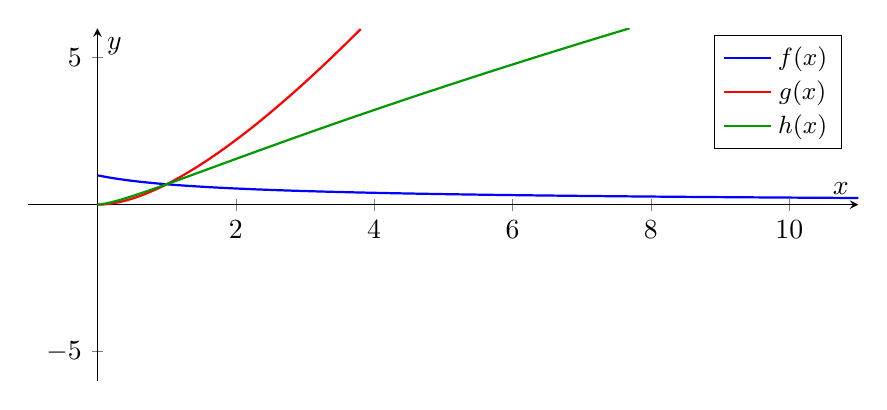
\begin{tikzpicture}
          \begin{axis}[
              axis lines = middle,
              xlabel = {$x$},
              ylabel = {$y$},
              xmin = -1, xmax = 11,
              ymin = -6, ymax = 6,
              samples = 400,
              width=\linewidth, height=0.5\linewidth,
              legend style={
                at={(0.98,0.98)}, anchor=north east, font=\small, fill=white
              },
              restrict y to domain=-6:6,
              unbounded coords=jump,
              clip mode=individual,
            ]

            \addplot[blue, thick, domain=0.001:11] {ln(1+x)/x};
            \addlegendentry{$f(x)$}

            \addplot[red, thick, domain=0:11] {x*ln(1+x)};
            \addlegendentry{$g(x)$}

            \addplot[green!60!black, thick, domain=0:11] {sqrt(x)*ln(1+x)};
            \addlegendentry{$h(x)$}

          \end{axis}
        \end{tikzpicture}
      \end{center}

      \textbf{(a)}

      $f(x)$ has a limit of 1 as the function approaches 0. This is because this function is essentially the same as $\tfrac{1}{x}\log(1+x)$. In this scenario, $\tfrac{1}{x}$ has a limit that rapidly approaches $+\infty$ and $\log(x+1)$ has a limit that approaches 0. There is a restriction $x > -1$, because of the restriction set by the logarithm. Then, the function seems to be dominated by $\tfrac{1}{x}$, as initial trends of the graph appear similarly to $\tfrac{1}{x}$. $\tfrac{1}{x}$ has a point at $(1,1)$, and this graph has a horizontal translation in value, moving it 1 value to the left. Therefore, that point which was previously $(1,1)$ becomes $(0,1)$.

      \hrule

      For $g(x)$: The function approaches 0 as $x \to 0^{+}$, as it has a horizontal asymptote at $x=0$. For any function that is continuous, the limit of $x$ as it approaches $a$ equals $g(a)$; therefore, we can plug in the value and know that it is the function’s limit.

      \[
        g(0) = 0\log(1+0) = 0
      \]

      \hrule

      For $h(x)$: The function approaches 0 as $x \to 0^{+}$. For any continuous function, if $g(0)=0$, then the limit as it approaches 0 is 0.

      \[
        h(x) = \sqrt{0}\,\log(1+0) = 0
      \]

      However, as $\sqrt{x}$ is undefined if $x<0$, the function $h(x)$ is not defined if $x<0$. Therefore, if we were to approach 0 from the left, we would find that it does not exist. The combined approach of 0 does not exist, but it exists when it approaches 0 from the right.

      \begin{center}
        \begin{tabular}{@{}l@{}}
          $\displaystyle \lim_{x \to 0} \sqrt{x}\log(1+x)$ \\[6pt]
          $\displaystyle = \sqrt{0}\log(1+0)$ \\[6pt]
          $\displaystyle = 0\log(1+0)$ \\[6pt]
          $\displaystyle = 0$ \\[6pt]
        \end{tabular}
      \end{center}

      \textbf{(b)}

      $f(x)$ approaches zero as $x$ approaches infinity as $\log(1+x)$ increases at a slower rate than $x$. Therefore, the denominator of $f(x)$ would increase at a higher rather than the numerator as $x$ approaches infinity, making $f(x)$ reach zero.

      $g(x)$ $(\infty)\log(1+x) = +\infty$ Therefore, as $x$ approaches infinity, the function $f(x)$ will infinitely grow without bound. In $g(x)$, the $x$ term grows at a constant slope of $1$ towards $+\infty$, while $\log_{e}(1+x)$ does to same, although at a smaller rate. Both terms are multiplied, leading the function to grow similar to a linear function.

      $h(x)$ $\sqrt{\infty}\cdot\log(1+\infty)=\infty$ The function grows infinitely, but at a slower rate than $g(x)$ since it is still a radical graph. The growth infinitely slows down but still infinitely increases, which is quite different from $g(x)$, where the growth gets faster.

      \textbf{(c)}

      \begin{center}
        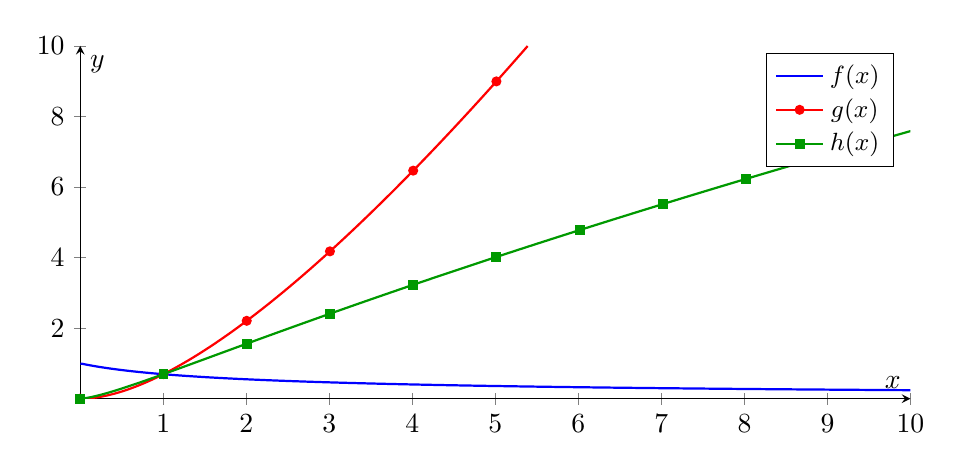
\begin{tikzpicture}
          \begin{axis}[
              axis lines = middle,
              xlabel = {$x$},
              ylabel = {$y$},
              xmin = 0, xmax = 10,
              ymin = 0, ymax = 10,
              samples = 400,
              width=\linewidth, height=0.5\linewidth,
              legend style={
                at={(0.98,0.98)}, anchor=north east, font=\small, fill=white
              },
              restrict y to domain=0:10,
              unbounded coords=jump,
              clip mode=individual,
            ]

            % f(x) = ln(1+x)/x  (avoid x=0)
            \addplot[blue, thick, domain=0.001:10] {ln(1+x)/x};
            \addlegendentry{$f(x)$}

            % g(x) = x*ln(1+x)  (solid red with occasional markers to distinguish)
            \addplot[red, thick, mark=*, mark repeat=40, mark options={solid,scale=0.7}, domain=0:10] {x*ln(1+x)};
            \addlegendentry{$g(x)$}

            % h(x) = sqrt(x)*ln(1+x)  (solid green with different marker)
            \addplot[green!60!black, thick, mark=square*, mark repeat=40, mark options={solid,scale=0.7}, domain=0:10] {sqrt(x)*ln(1+x)};
            \addlegendentry{$h(x)$}

          \end{axis}
        \end{tikzpicture}
      \end{center}

      h(x)’s growth is rapid then slows down like the logarithmic parent function. g(x)’s has steadier growth near small x values, then grows faster towards large x values.

    \end{solution}

    \hrulefill

    \question \pts[5]
    \textbf{Contest A (Small $x$):} Rank the following as $x\to 0^+$ and describe behaviours (tend to $0$, $\pm\infty$, finite constant; sign; speed of vanishing/divergence):
    \[
      f_1(x)=x\log x,\quad
      f_2(x)=\log(\log x),\quad
      f_3(x)=e^x,\quad
      f_4(x)=\sqrt{x},\quad
      f_5(x)=e^{\sqrt{x}},\quad
      f_6(x)=x^{10},\quad
      f_7(x)=\log x.
    \]
    Include a short note on \emph{domain} near $0$ and a graph on $(0,0.5]$ that helps you compare the functions that remain finite.

    % Q4
    \begin{solution}
      \begin{center}
        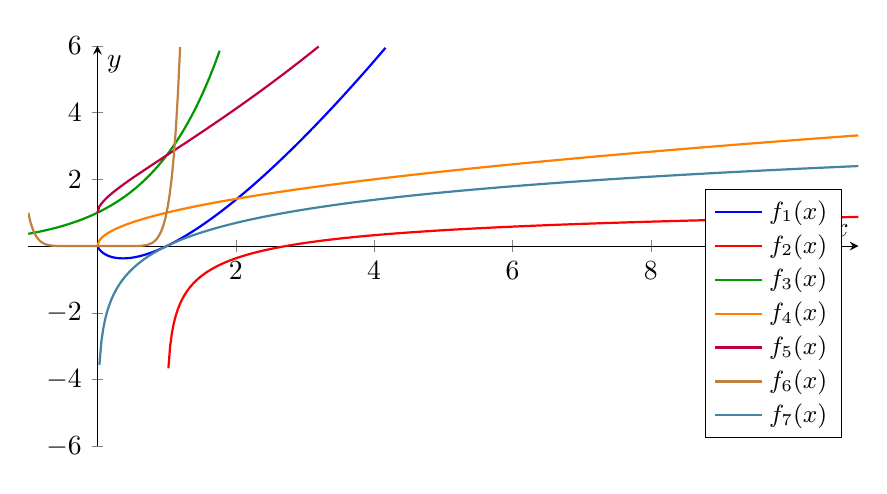
\begin{tikzpicture}
          \begin{axis}[
              axis lines = middle,
              xlabel = {$x$},
              ylabel = {$y$},
              xmin = -1, xmax = 11,
              ymin = -6, ymax = 6,
              samples = 400,
              width=\linewidth, height=0.55\linewidth,
              legend style={
                at={(0.98,0.02)}, anchor=south east, font=\small, fill=white
              },
              restrict y to domain=-6:6,
              unbounded coords=jump,
              clip mode=individual,
            ]

            \addplot[blue, thick, domain=0.001:11] {x*ln(x)};
            \addlegendentry{$f_{1}(x)$}

            \addplot[red, thick, domain=1.001:11] {ln(ln(x))};
            \addlegendentry{$f_{2}(x)$}

            \addplot[green!60!black, thick, domain=-1:11] {exp(x)};
            \addlegendentry{$f_{3}(x)$}

            \addplot[orange, thick, domain=0:11] {sqrt(x)};
            \addlegendentry{$f_{4}(x)$}

            \addplot[purple, thick, domain=0:11] {exp(sqrt(x))};
            \addlegendentry{$f_{5}(x)$}

            \addplot[brown, thick, domain=-1:11] {x^10};
            \addlegendentry{$f_{6}(x)$}

            \addplot[cyan!60!black, thick, domain=0.001:11] {ln(x)};
            \addlegendentry{$f_{7}(x)$}

          \end{axis}
        \end{tikzpicture}
      \end{center}

      \textbf{$f_1(x)$}

    3.) This graph approaches $0$ when $x$ approaches $0$ from the right. This can be seen on the graph and can also be found algebraically by setting $x=0$ in the function. We know this is only true when $x$ approaches $0$ from the right as $\log(x)$ is undefined when $x<0$. Therefore, the limit for the function when $x$ approaches $0$ from the left does not exist. It vanishes faster than $x\log(x)$ since $\dfrac{x\log(x)}{\sqrt{x}}$ is equal to $0$ when it approaches $0$ from the right, not infinity. This is the formula used to calculate speed of vanishing.

    \textbf{$f_2(x)$}

  7.) We can say that this graph does not even have a limit as $x$ approaches $0$ from the right, as the function only exists when $x>1$, and has a limit at $x=1$. $\lim_{x \to 0^+}$ DNE. Therefore, it will not easily dominate small $x$, as it does not approach $0$ at all. The reason that $\log(\log(x))$ is undefined is since $x$ must be greater than $1$ (because $\log(1)=0$), and if the inner $\log(x)$ is equal to $0$, then the outer log becomes undefined.

  \textbf{$f_3(x)$}

2.) This graph approaches $1$ when $x$ approaches $0$ from the right. This can be seen on the graph and can also be found algebraically by setting $x=0$ in the function. This will be the case for essentially any graph to the power of $x$ without a vertical or horizontal translation, since anything to the power of $0$ is equal to $1$.

\textbf{$f_4(x)$}

4.) This graph approaches $0$ when $x$ approaches $0$ from the right. This can be seen on the graph and can also be found algebraically by setting $x=0$ in the function. We know this is only true when $x$ approaches $0$ from the right as $\sqrt{x}$ is undefined when $x<0$. Therefore, the limit for the function when $x$ approaches $0$ from the left does not exist. This graph vanishes slower than $x\log(x)$ since $\dfrac{x\log(x)}{\sqrt{x}}$ is equal to $0$ when it approaches $0$ from the right, not infinity.

\textbf{$f_5(x)$}

1.) This graph approaches $1$ when $x$ approaches $0$ from the right. This can be seen on the graph and can also be found algebraically by setting $x=0$ in the function, as $e^{\sqrt{0}}=1$. We know this is only true when $x$ approaches $0$ from the right as $\sqrt{x}$ is undefined when $x<0$. Therefore, the limit for the function when $x$ approaches $0$ from the left does not exist.

\textbf{$f_6(x)$}

5.) The limit of this graph as $x$ approaches $0$ from the right is simply $0$; you can plug $0$ into the equation, and it will give the value $0$. For the graph of $x^{10}$, its decay towards $0$ will occur faster than lower power functions like $x^2$, but slower than higher power functions like $x^{11}$. In other words, it vanishes quite quickly.

\textbf{$f_7(x)$}

6.) This graph only exists for $x>0$, as this is the restriction for a $\log(x)$ graph. Therefore, the limit as $x$ approaches $0^+$ is $-\infty$.

\end{solution}

% -------------------------------------------------------

\question \pts[5]
\textbf{Contest B (Large $x$):} Rank the following from \emph{slowest} growth to \emph{fastest} growth as $x\to\infty$ and justify briefly. Include a graph on a domain that reveals the growth distinctions.
\[
f_1(x)=x\log x,\quad
f_2(x)=\log(\log x),\quad
f_3(x)=e^x,\quad
f_4(x)=\sqrt{x},\quad
f_5(x)=e^{\sqrt{x}},\quad
f_6(x)=x^{10},\quad
f_7(x)=\log x.
\]

% Q5
\begin{solution}

\begin{center}
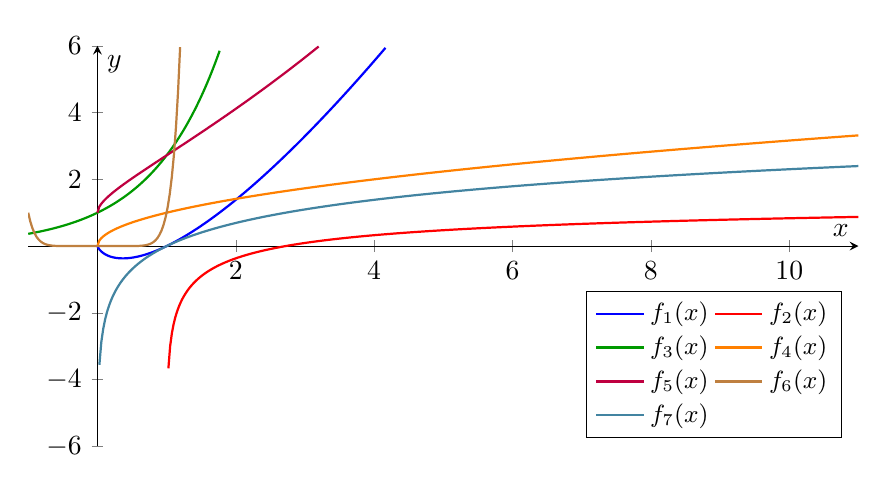
\begin{tikzpicture}
\begin{axis}[
axis lines = middle,
xlabel = {$x$},
ylabel = {$y$},
xmin = -1, xmax = 11,
ymin = -6, ymax = 6,
samples = 400,
width=\linewidth, height=0.55\linewidth,
legend style={
  at={(0.98,0.02)}, anchor=south east,
  font=\small, fill=white,
  legend columns=2
},
restrict y to domain=-6:6,
unbounded coords=jump,
clip mode=individual,
]

\addplot[blue, thick, domain=0.001:11] {x*ln(x)};
\addlegendentry{$f_{1}(x)$}

\addplot[red, thick, domain=1.001:11] {ln(ln(x))};
\addlegendentry{$f_{2}(x)$}

\addplot[green!60!black, thick, domain=-1:11] {exp(x)};
\addlegendentry{$f_{3}(x)$}

\addplot[orange, thick, domain=0:11] {sqrt(x)};
\addlegendentry{$f_{4}(x)$}

\addplot[purple, thick, domain=0:11] {exp(sqrt(x))};
\addlegendentry{$f_{5}(x)$}

\addplot[brown, thick, domain=-1:11] {x^10};
\addlegendentry{$f_{6}(x)$}

\addplot[cyan!60!black, thick, domain=0.001:11] {ln(x)};
\addlegendentry{$f_{7}(x)$}
\end{axis}
\end{tikzpicture}
\end{center}

\textbf{$f_1(x)$}

4.) This function on the infinite scale of things becomes nearly linear; therefore, the growth rate is not as high as it looks initially. The linear function $x$ dominates for big $x$, as $\log(x)$ grows at a very slow rate.

\textbf{$f_2(x)$}

1.) This function grows incredibly slowly as it approaches infinity, as the growth rate infinitely decreases (although still positive) as it approaches infinity. Big $x$ is dominated by $\log(x)$, and $\log(x)$ grows infinitely slowly. This happens even slower than a radical function, and a regular logarithmic function.

\textbf{$f_3(x)$}

7.) A graph of $e^x$ will overtake any function on the infinitely large scale of things, and therefore has the fastest growth as $x$ approaches infinity. For big $x$, nearly every function is dominated by $e^x$, as it has a very fast growth rate.

\textbf{$f_4(x)$}

3.) This radical function will infinitely increase, but the rate at which it increases will infinitely decrease, making the growth rate very slow.

\textbf{$f_5(x)$}

6.) A graph of $e^x$ will still overtake about any function not involving Euler’s number, since on the grand scale of things, Euler’s number to the power of any positive number will overtake nearly any other function, even though it initially grows slowly.

\textbf{$f_6(x)$}

5.) $x^{10}$ increases slowly for small $x$, but for big $x$ it increases infinitely.

\textbf{$f_7(x)$}

2.) This logarithmic function will increase infinitely, but plateau over time as the growth rate infinitely decreases, even though it is still positive. This will happen slower than a radical function, but faster than a $\log(\log(x))$ function.

\end{solution}

\hrulefill

\fullwidth{
\subsection*{Comparisons: }}
In the following questions, you will compare two functions on the regimes of small $x$ and large $x$. Be sure to consider the expectations for what to include given in the assignment setup.
\question \pts[4] Consider the functions
\[
f(x)=\frac{e^{\sqrt{x}}}{x^2},\qquad
g(x)=x\log(1+x).
\]
\begin{parts}
\part[2] Compare $f(x)$ and $g(x)$ as $x\to 0^+$.
\part[2] Compare $f(x)$ and $g(x)$ as $x\to\infty$.
\end{parts}

% Q6
\begin{solution}

\begin{center}
\begin{tikzpicture}
\begin{axis}[
width=12cm, height=8cm,
axis lines=middle,
xlabel={$x$}, ylabel={$y$},
xmin=-1, xmax=11,
ymin=-6, ymax=6,
domain=-1:11,
samples=400,
legend style={at={(1,1)}, anchor=north east},
restrict y to domain=-6:6,
unbounded coords=jump,
clip mode=individual,
]

\addplot[blue, thick, domain=-1:11, samples=400] {exp(sqrt(x))/x^2};
\addlegendentry{$f(x)$}

\addplot[red, thick, domain=-1:11, samples=400] {x*ln(1+x)};
\addlegendentry{$g(x)$}

\end{axis}
\end{tikzpicture}
\end{center}

\textbf{(a)}

For the numerator on $f(x)$, at $x \to 0^{+}$, $\sqrt{x}$ reaches $0$, and $e^{0}=1$. As for the denominator, $x^{2}$ reaches a very small positive number. This makes the simplified $f(x)$ equal to $\frac{1}{\text{small positive number}}$. This signifies positive growth towards the vertical asymptote at $x=0$.

\hrule

The function $g(x)$ approaches zero as $x$ reaches zero since $g(0)$ is equal to zero, and for any continuous function, if $g(0)=0$, then the limit as it approaches $0$ is $0$.

$\therefore f(x)$ and $g(x)$ have opposite behaviours as they reach the limit. As $x \to 0^{+}$, $f(x)$ reaches $+$ while $g(x)$ reaches $0$.

\textbf{(b)}

The function $f(x)$ approaches infinity as $x$ approaches infinity. This is because $f(x)$ is comprised of an exponential function divided by a polynomial function. The rate of which an exponential function increases is higher than that of a polynomial function, causing the numerator to increase at a higher rate than the denominator and allowing $f(x)$ to reach infinity.

\hrule

The function $g(x)$ approaches infinity as $x$ approaches infinity. This is because $g(\infty)=\infty$.

$\vspace{1pt}$

$\therefore$ $f(x)$ and $g(x)$ have opposite behaviours as they approach the limit. As $x \to \infty$, $f(x)$ reaches $0$ while $g(x)$ reaches infinity.

\end{solution}

% -------------------------------------------------------

\question \pts[4] Consider the functions
\[
f(x)=\frac{x^3+e^x}{x^2+e^{\sqrt{x}}},\qquad
g(x)=\frac{\log(1+x)}{x}.
\]
\begin{parts}
\part[2] Compare the behaviours of $f(x)$ and $g(x)$ as $x\to 0^+$.
\part[2] Compare the behaviours of $f(x)$ and $g(x)$ as $x\to\infty$.
\end{parts}

% Q7
\begin{solution}
\begin{center}
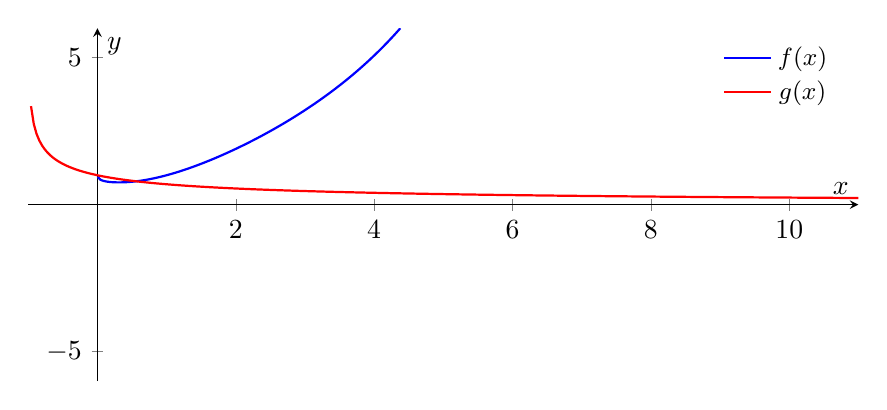
\begin{tikzpicture}
\begin{axis}[
axis lines = middle,
xlabel = {$x$},
ylabel = {$y$},
xmin = -1, xmax = 11,
ymin = -6, ymax = 6,
samples = 300,
width=\linewidth, height=0.5\linewidth,   % <-- fit to available width
legend style={
at={(0.98,0.98)}, anchor=north east, font=\small, draw=none, fill=white
},
restrict y to domain=-6:6,
unbounded coords=jump,
clip mode=individual,
]

\addplot[blue, thick, domain=-1:11] {(x^3 + exp(x))/(x^2 + exp(sqrt(x)))};
\addlegendentry{$f(x)$}

\addplot[red, thick, domain=-1:11] {ln(1+x)/x};
\addlegendentry{$g(x)$}

\end{axis}
\end{tikzpicture}
\end{center}

\textbf{(a)}
For small $x$ values, the dominant terms for $f(x)$ are $e^x$ and $e^{x\sqrt{x}}$. Therefore, removing $x^n$ makes negligible difference. Approaching $0^{+}$, $x^n$ plateaus towards $0$ while $e^x$ and $e^{x\sqrt{x}}$ grow towards $1$ at small $x$ values. This makes the latter the dominant term. Since I know $e^x$ grows faster than $e^{\sqrt{x}}$ (and they're equal at 1), this means the function approaches $1$ as $x$ approaches $0$ from the right.

\begin{center}
\begin{tabular}{@{}l@{}}
$\displaystyle \lim_{x \to 0}\frac{x^3+e^x}{x^2+e^{\sqrt{1}}}$ \\[10pt]
$\displaystyle \lim_{x \to 0}\frac{0+1}{0+1} = 1$ \\[6pt]
\end{tabular}
\end{center}

\hrule

As for $g(x)$, we can use squeeze theorem to solve the limit as $x$ approaches $0^+$.

\begin{center}
\begin{tabular}{@{}l@{}}
$\displaystyle \frac{1}{x} (\frac{x}{1+x}) \le \frac{\log(1+x)}{x} \le \frac{x}{x}$ \\[6pt]
$\displaystyle \frac{1}{1+x} \le \frac{\log(1+x)}{x} \le 1$ \\[6pt]
$\displaystyle \lim_{x \to 0^{+}} \frac{\log(1+x)}{x} = \frac{\log(1+0)}{0} = 1$ \\[6pt]
\end{tabular}
\end{center}

$\therefore f(x)$ and $g(x)$ grow towards $1$ at the limit.

\textbf{(b)}
Again, analyzing $f(x)$ with the $nx$ terms removed, I know $e^x$ grows faster than $e^{\sqrt{x}}$, which means as it approaches the limit infinity, it grows towards positive infinity. $g(x)$ is equal to $\frac{1}{x}\log(x+1)$. When considering which function dominates for big $x$ vs. small $x$, we consider the rate of growth vs. the rate of decay, not simply whether it is growing or decaying. The logarithmic function for big $x$ grows, but at an infinitely slow rate. In contrast, the graph of $1/x$ decays at a very quick rate as $x$ approaches infinity. Because this rate is larger, big $x$ is dominated by $1/x$ rather than $\log(x+1)$, AND $1/x$ infinitely approaches $0$. $\therefore g(x)$ infinitely approaches $0$. This is similar to how any function being divided by $e^x$ will be dominated by $1/e^x$ since the decay rate is so large; we are looking at the rate, rather than whether it is growing or decaying.

$\therefore f(x)$ grows while $g(x)$ decays at the limit of $x$ as it approaches infinity. $f(x)$ grows much faster.

\end{solution}

%     -------------------------------------------------------

\question \pts[4] Consider the functions
\[
f(x)=x^2\log(1+x),\qquad
g(x)=e^{\sqrt{x}}-x.
\]
\begin{parts}
\part[2] Compare $f(x)$ and $g(x)$ as $x\to 0^+$.
\part[2] Compare $f(x)$ and $g(x)$ as $x\to\infty$.
\end{parts}

% Q8
\begin{solution}
\begin{center}
\begin{tikzpicture}
\begin{axis}[
axis lines = middle,
xlabel = {$x$},
ylabel = {$y$},
xmin = 0, xmax = 11,
ymin = -6, ymax = 6,
samples = 400,
width=0.9\textwidth, height=0.45\textwidth,
legend style={
at={(0.98,0.98)}, anchor=north east, font=\small, draw=none, fill=white
},
restrict y to domain=-6:6,
unbounded coords=jump,
clip mode=individual,
]

\addplot[blue, thick, domain=0:11] {x^2 * ln(1+x)};
\addlegendentry{$f(x)$}

\addplot[red, thick, domain=0:11] {exp(sqrt(x)) - x};
\addlegendentry{$g(x)$}

\end{axis}
\end{tikzpicture}
\end{center}

\textbf{(a)}
As $x$ approaches $0^+$, $f(x)$ approaches $0$.

\begin{center}
\begin{tabular}{@{}l@{}}
$\displaystyle \lim_{x \to 0} \log(1+x) = 0^2$ \\[6pt]
$\displaystyle \lim_{x \to 0} \log(1+0) = 0$ \\[6pt]
$\displaystyle \lim_{x \to 0} \log(1) = 0$ \\[6pt]
\end{tabular}
\end{center}

\hrule

As $x$ approaches $0^+$, $g(x)$ approaches $1$.

\begin{center}
\begin{tabular}{@{}l@{}}
$\displaystyle \lim_{x \to 0} e^{\sqrt{x}}-x$ \\[6pt]
$\displaystyle = e^{\sqrt{10}}-0$ \\[6pt]
$\displaystyle = e^0 -0$ \\[6pt]
$\displaystyle = 1 - 0$ \\[6pt]
$\displaystyle = 1$ \\[6pt]
\end{tabular}
\end{center}

\textbf{(b)}
As $x$ approaches infinity, $f(x)$ approaches infinity. This is because $\log(1+x)$ has an incredibly slow growth rate when considering big $x$, so it is completely dominated by $x^2$, which has quite a large growth rate. Therefore, the function not only approaches infinity, but grows without bound. For the record, both $\log(x+1)$ and $x^2$ would approach infinity as the limit approaches infinity to begin with; $x^2$ however, does so at a much faster rate.

\hrule

As $x$ approaches infinity, $g(x)$ approaches infinity; furthermore, it approaches infinity with a growth rate similar to that of $e^{\sqrt{x}}$. This is because in this function, as the limit of $x$ approaches infinity, $x$ is completely dominated by $e^{\sqrt{x}}$ since Euler’s number, even to the power of the root of $x$, grows at an incredibly fast rate as $x$ approaches infinity. Since it grows much faster than $x$, and nearly any other function, it will dominate the function for big $x$, and it will grow in an $e^{\sqrt{x}}$ rate.

$\therefore g(x)$ grows faster than $f(x)$ as $x$ approaches infinity. From what you can tell from the graph it looks as if $f(x)$ grows faster than $g(x)$, and it does initially, but on the infinite scale of things, $e^{\sqrt{x}}$ will overtake nearly any function. Therefore, $g(x)$ grows faster than $f(x)$.
\end{solution}

% -------------------------------------------------------

\question \pts[4] Consider the functions
\[
f(x)=\frac{\sin(x^2)}{x},\qquad
g(x)=\frac{1+\log(1+x)}{1+x}.
\]
\begin{parts}
\part[2] Compare the behaviours of $f(x)$ and $g(x)$ as $x\to 0$.
\part[2] Compare the behaviours of $f(x)$ and $g(x)$ as $x\to\infty$.
\end{parts}

% Q9
\begin{solution}
\textbf{(a)}
As $x$ approaches $0^+$, $f(x)$ approaches $0$. From the start, we know that the value of this graph cannot exceed $1/x$, or $–1/x$, as is dictated by the amplitude term since this equation is the same as $(1x)(sin(x^2))$. To solve this limit, we need get to a point where we can use the identity $\frac{\sin{x}}{x}$ as the limit approaches $0$ is equal to $1$. We can multiple an $x$ into both the numerator and denominator to get to this point, and then simplify. When we do this, we find that the function as the limit approaches $0$ is equal to $(x)(1)$ or simply $x$. $\therefore$ we can plug-in the limit and solve, finding that it is equal to 0.

\begin{center}
\begin{tabular}{@{}l@{}}
$\displaystyle \lim_{x \to 0} \frac{\sin(x^2)}{x}$ \\[6pt]
$\displaystyle = \lim_{x \to 0} \frac{\sin(x^2)}{x} \cdot \frac{x}{x}$ \\[6pt]
$\displaystyle = \lim_{x \to 0} x\frac{\sin(x^2)}{x^2}$ \\[6pt]
$\displaystyle = \lim_{x \to 0} x(1)$ \\[6pt]
$\displaystyle = \lim_{x \to 0} (0)(1)=0$ \\[6pt]
$\displaystyle \therefore \lim_{x \to 0^+} \frac{\sin(x^2)}{x}=0$ \\[6pt]
\end{tabular}
\end{center}

\hrule
As $x$ approaches $0^+$, $g(x)$ approaches $1$. Using direct substitution, you end up with $\frac{1+\log{1}}{1})=1$. For any function that is continuous, the limit of $g(x)$ as $x$ approaches a will be equal to $g(a)$, and if the limit exists for $0$, than it is equal to the limit of zero from the right. Furthermore, the reason that this graph has a y-intercept unlike most logarithmic graphs is because it has a horizontal translation value of $1$ to the left, making it approach $-\infty$ at the limit of $–1^+$ instead of $0^+$.

\begin{center}
\begin{tabular}{@{}l@{}}
$\displaystyle \lim_{x \to 0} \frac{1+\log(1+x)}{1+x}$ \\[6pt]
$\displaystyle = \frac{1+\log(1+0)}{1+0}$ \\[6pt]
$\displaystyle = \frac{1}{1}$ \\[6pt]
$\displaystyle = 1$ \\[6pt]
\end{tabular}
\end{center}

\textbf{(b)}
As $x$ approaches $\infty$, $f(x)$ approaches 0. We know this because we can apply the squeeze theorem; we know that the function oscillates between $-1/x$ and $1/x$. As the function approaches infinity, these become $0$. If the function is squeezed by an oscillation of $0$ on either side, it infinitely approaches $0$.

\begin{center}
\begin{tabular}{@{}l@{}}
$\displaystyle -1 \le \sin(x) \le 1$ \\[6pt]
$\displaystyle -1 \le \sin(x^2) \le 1$ \\[6pt]
$\displaystyle \frac{-1}{x} \le \frac{\sin(x^2)}{x} \le \frac{1}{x}$ \\[6pt]
$\displaystyle \frac{-1}{\infty} \le \frac{\sin(\infty^2)}{\infty} \le \frac{1}{\infty}$ \\[6pt]
$\displaystyle 0 \le \frac{\sin(\infty^2)}{\infty} \le 0$ \\[6pt]
$\displaystyle = \lim_{x \to \infty} \frac{\sin(x^2)}{x} = 0$ \\[6pt]
\end{tabular}
\end{center}

\hrule

As x approaches infinity, g(x) approaches 0. We know that as x approaches infinity, log(x)/x is equal to 0. This is because the growth rate of a logarithmic function is so much slower than the growth rate of a linear function on the infinite scale that the numerator is outgrown by the denominator, making the limit equal to 0 as the function approaches infinity. Since log(x+1)/x is so similar, and the +1 is negligible when working with infinity, we know the limit as this approaches infinity is 0 as well. Therefore, we can manipulate the limit in this fashion to prove it:

\begin{center}
\begin{tabular}{@{}l@{}}
$\displaystyle \lim_{x \to \infty} \frac{1+log(1+x)}{1+x}$ \\[6pt]
$\displaystyle = \lim_{x \to \infty} \frac{1}{1+x} + \frac{log(1+x)}{1+x}$ \\[6pt]
$\displaystyle = \lim_{x \to \infty} \frac{1}{1+x} + 0$ \\[6pt]
$\displaystyle = \lim_{x \to \infty} \frac{1}{1+\infty} + 0$ \\[6pt]
$\displaystyle = \lim_{x \to \infty} 0 + 0$ \\[6pt]
$\displaystyle = \lim_{x \to \infty} 0 + 0$ \\[6pt]
\end{tabular}
\end{center}

\end{solution}

% -------------------------------------------------------
\question \pts[4] Consider the functions
\[
f(x)=\frac{\log(e^x+x^2)}{x},\qquad
g(x)=\frac{\log(1+x^2)}{\sqrt{x}}.
\]
\begin{parts}
\part[2] Compare $f(x)$ and $g(x)$  as $x\to 0^+$.
\part[2] Compare $f(x)$ and $g(x)$ as $x\to\infty$.
\end{parts}

% Q10
\begin{solution}

\begin{center}
\begin{tikzpicture}
\begin{axis}[
width=12cm, height=8cm,
axis lines=middle,
xlabel={$x$}, ylabel={$y$},
xmin=-1, xmax=11,
ymin=-6, ymax=6,
domain=-1:11,
samples=200,
legend style={at={(1,1)}, anchor=north east}
]

\addplot[blue, thick] {ln(exp(x) + x^2)/x};
\addlegendentry{$f(x)$}

\addplot[red, thick, domain=-1:11] {ln(1 + x^2)/sqrt(x)};
\addlegendentry{$g(x)$}

\end{axis}
\end{tikzpicture}
\end{center}

\textbf{(a)}

For $f(x)$, we can use squeeze theorem to solve the limit as $x$ approaches $0^+$.

Since $e^{x}$ approaches $1$ at the limit compared to $x^{2}$ approaching $0$, it dominates ($1+0=1$). $\therefore f(x)$’s numerator can be simplified as $\ln(e^{x})$, which equals $x$. Using my mathematical intuition, I know $\frac{x}{x}$ creates a horizontal line at $x=1$, but is undefined at $x=0$ due to division by 0. However, I can use this information to solve the limit as:

\begin{center}
\begin{tabular}{@{}l@{}}
$\displaystyle \lim_{x \to 0^+} \frac{\log(e^x+x^2)}{x}$ = 1\\[6pt]
\end{tabular}
\end{center}

\hrule

Using my intuitive knowledge of calculus, I know that $\log_{e}(1+u)=u$. With this inequality and squeeze theorem, I can set up the following:

\begin{center}
\begin{tabular}{@{}l@{}}
$ 0 \le \frac{\log(1+x^{2})}{\sqrt{x}} \leq \frac{x^{2}}{\sqrt{2}} = x^{3/2} $\\[6pt]
\end{tabular}
\end{center}

Finally, I can use direct substitution to solve how the limit of $g(x)$ as $x \to 0^{+}$. (It goes towards $0$).

\[
0^{3/2} = 0
\]

\textbf{(b)}

Similarly with $f(x)$, $e^{x}$ dominates over $x^{2}$. This time, it is because its exponential growth is much larger than the polynomial growth. This means its numerator can again be simplified as $\ln(e^{x})$, which equals $x$. $\therefore f(x)$ also equals $1$ as it approaches infinity.

\hrule

As for big $x$ values, the positive $1$ term in the numerator is irrelevant, leading $g(x)$ to be simplified as

\[
\frac{\log_{e}(1+x^{2})}{\sqrt{x}}
\]

\[
= \frac{2\log_{e}(1+x)}{\sqrt{x}}
\]

I know $\log_{e}{x}$ grows slower than any form of $x^{1/n}$ where $n$ is a positive number. $\therefore g(x)$ equals $0$ as it approaches infinity.

\end{solution}

\hrulefill

\fullwidth{
\subsection*{Reporting}}

For each problem, include (i) concise explanations in complete sentences, (ii) at least one graph that illuminates your conclusions, and (iii) a brief summary sentence stating which function(s) dominate in each regime and why (in terms of dominant terms).

\end{questions}

\hrulefill

\end{document}

%-------------------------------------------------------------
%-------------------------------------------------------------
%-------------------------------------------------------------
